%package list
\documentclass{article}
\usepackage[top=3cm, bottom=3cm, outer=3cm, inner=3cm]{geometry}
\usepackage{multicol}
\usepackage{graphicx}
\usepackage{url}
%\usepackage{cite}
\usepackage{hyperref}
\usepackage{array}
%\usepackage{multicol}
\newcolumntype{x}[1]{>{\centering\arraybackslash\hspace{0pt}}p{#1}}
\usepackage{natbib}
\usepackage{pdfpages}
\usepackage{multirow}
\usepackage[normalem]{ulem}
\useunder{\uline}{\ul}{}
\usepackage{svg}
\usepackage{xcolor}
\usepackage{listings}
\lstdefinestyle{ascii-tree}{
    literate={├}{|}1 {─}{--}1 {└}{+}1 
  }
\lstset{basicstyle=\ttfamily,
  showstringspaces=false,
  commentstyle=\color{red},
  keywordstyle=\color{blue}
}
%\usepackage{booktabs}
\usepackage{caption}
\usepackage{subcaption}
\usepackage{float}
\usepackage{array}

\newcolumntype{M}[1]{>{\centering\arraybackslash}m{#1}}
\newcolumntype{N}{@{}m{0pt}@{}}


%%%%%%%%%%%%%%%%%%%%%%%%%%%%%%%%%%%%%%%%%%%%%%%%%%%%%%%%%%%%%%%%%%%%%%%%%%%%
%%%%%%%%%%%%%%%%%%%%%%%%%%%%%%%%%%%%%%%%%%%%%%%%%%%%%%%%%%%%%%%%%%%%%%%%%%%%
\newcommand{\itemEmail}{rcompanocca@unsa.edu.pe}
\newcommand{\itemStudent}{Roni Companocca Checco}
\newcommand{\itemCourse}{Programación}
\newcommand{\itemCourseCode}{20210558}
\newcommand{\itemSemester}{II}
\newcommand{\itemUniversity}{Universidad Nacional de San Agustín de Arequipa}
\newcommand{\itemFaculty}{Facultad de Ingeniería de Producción y Servicios}
\newcommand{\itemDepartment}{Departamento Académico de Ingeniería de Sistemas e Informática}
\newcommand{\itemSchool}{Escuela Profesional de Ingeniería de Sistemas}
\newcommand{\itemAcademic}{2023 - B}
\newcommand{\itemInput}{Del 28 octubre 2023}
\newcommand{\itemOutput}{Al 2 Noviembre 2023}
\newcommand{\itemPracticeNumber}{12}
\newcommand{\itemTheme}{Definición de Clases de Usuario Clase Soldado - Menú}
%%%%%%%%%%%%%%%%%%%%%%%%%%%%%%%%%%%%%%%%%%%%%%%%%%%%%%%%%%%%%%%%%%%%%%%%%%%%
%%%%%%%%%%%%%%%%%%%%%%%%%%%%%%%%%%%%%%%%%%%%%%%%%%%%%%%%%%%%%%%%%%%%%%%%%%%%

\usepackage[english,spanish]{babel}
\usepackage[utf8]{inputenc}
\AtBeginDocument{\selectlanguage{spanish}}
\renewcommand{\figurename}{Figura}
\renewcommand{\refname}{Referencias}
\renewcommand{\tablename}{Tabla} %esto no funciona cuando se usa babel
\AtBeginDocument{%
	\renewcommand\tablename{Tabla}
}

\usepackage{fancyhdr}
\pagestyle{fancy}
\fancyhf{}
\setlength{\headheight}{30pt}
\renewcommand{\headrulewidth}{1pt}
\renewcommand{\footrulewidth}{1pt}
\fancyhead[L]{\raisebox{-0.2\height}{
\includegraphics[width=3cm]{logo_episunsa.png}}}
\fancyhead[C]{\fontsize{7}{7}\selectfont	\itemUniversity \\ \itemFaculty \\ \itemDepartment \\ \itemSchool \\ \textbf{\itemCourse}}
\fancyhead[R]{\raisebox{-0.2\height}{
\includegraphics[width=1.2cm]{abet.png}}}
\fancyfoot[L]{Estudiante Roni Companocca Checco}
\fancyfoot[C]{\itemCourse}
\fancyfoot[R]{Página \thepage}

% para el codigo fuente
\usepackage{listings}
\usepackage{color, colortbl}
\definecolor{dkgreen}{rgb}{0,0.6,0}
\definecolor{gray}{rgb}{0.5,0.5,0.5}
\definecolor{mauve}{rgb}{0.58,0,0.82}
\definecolor{codebackground}{rgb}{0.95, 0.95, 0.92}
\definecolor{tablebackground}{rgb}{0.8, 0, 0}

\lstset{frame=tb,
	language=bash,
	aboveskip=3mm,
	belowskip=3mm,
	showstringspaces=false,
	columns=flexible,
	basicstyle={\small\ttfamily},
	numbers=none,
	numberstyle=\tiny\color{gray},
	keywordstyle=\color{blue},
	commentstyle=\color{dkgreen},
	stringstyle=\color{mauve},
	breaklines=true,
	breakatwhitespace=true,
	tabsize=3,
	backgroundcolor= \color{codebackground},
}

\begin{document}
	
	\vspace*{10px}
	
	\begin{center}	
		\fontsize{17}{17} \textbf{ Informe de Laboratorio \itemPracticeNumber}
	\end{center}
	\centerline{\textbf{\Large Tema: \itemTheme}}
	%\vspace*{0.5cm}	

	\begin{flushright}
		\begin{tabular}{|M{2.5cm}|N|}
			\hline 
			\rowcolor{tablebackground}
			\color{white} \textbf{Nota}  \\
			\hline 
			     \\[30pt]
			\hline 			
		\end{tabular}
	\end{flushright}	

	\begin{table}[H]
		\begin{tabular}{|x{4.7cm}|x{4.8cm}|x{4.8cm}|}
			\hline 
			\rowcolor{tablebackground}
			\color{white} \textbf{Estudiante} & \color{white}\textbf{Escuela}  & \color{white}\textbf{Asignatura}   \\
			\hline 
			{\itemStudent \par \itemEmail} & \itemSchool & {\itemCourse \par Semestre: \itemSemester \par Código: \itemCourseCode}     \\
			\hline 			
		\end{tabular}
	\end{table}		
	
	\begin{table}[H]
		\begin{tabular}{|x{4.7cm}|x{4.8cm}|x{4.8cm}|}
			\hline 
			\rowcolor{tablebackground}
			\color{white}\textbf{Laboratorio} & \color{white}\textbf{Tema}  & \color{white}\textbf{Duración}   \\
			\hline 
			\itemPracticeNumber & \itemTheme & 04 horas   \\
			\hline 
		\end{tabular}
	\end{table}
	
	\begin{table}[H]
		\begin{tabular}{|x{4.7cm}|x{4.8cm}|x{4.8cm}|}
			\hline 
			\rowcolor{tablebackground}
			\color{white}\textbf{Semestre académico} & \color{white}\textbf{Fecha de inicio}  & \color{white}\textbf{Fecha de entrega}   \\
			\hline 
			\itemAcademic & \itemInput &  \itemOutput  \\
			\hline 
		\end{tabular}
	\end{table}

    \section{TAREA}
	\begin{itemize}	
    \subsection{Objetivos:}
		\item Que el alumno demuestre poder crear  “clases definidas por el programador” 
		\item Implementar métodos para las clases definidas por el programador
       
    \subsection{Competencias a alcanzar:}
		\item Diseña, responsablemente, sistemas, componentes o procesos para satisfacer necesidades dentro de restricciones realistas: económicas, medio ambientales, sociales, políticas, éticas, de salud, de seguridad, manufacturación y sostenibilidad.
        \item Aplica de forma flexible, técnicas, métodos, principios, normas, estándares y herramientas de ingeniería necesarias para la construcción de software e implementación de sistemas de información.
    \subsection{Marco teorico:}
        \item Clase: Una Fábrica de objetos. Una clase está conformada por dos partes: datos miembro (variables de instancia / atributos) y los métodos. 
        \item Los métodos nos permiten acceder y/o modificar los datos miembros (atributos) de los objetos. 
        \item Toda clase necesita al menos un Constructor. El constructor lleva el mismo nombre de la clase. El constructor es un método especial que siempre se llama con la palabra reservada new() 
        
    \subsection{Indicaciones generales:}
        \item Todos los ejercicios deberán ser guardados en el mismo Proyecto
        \item El Proyecto deberá tener el nombre del Laboratorio y el nombre del alumno, así por ejemplo: Laboratorio 1 – Juan Perez
        \item Cada Clase deberá tener el nombre del ejercicio, así por ejemplo: Ejercicio1
        \item Utilice nombres de variables significativos y todas las recomendaciones de estilo
        \item Especialmente, su código deberá estar correctamente indentado
        \item Deberá pasar TODOS los casos de prueba
	\end{itemize}

    \section{EQUIPOS, MATERIALES Y TEMAS UTILIZADOS}
	\begin{itemize}
		\item Sistema Operativo Windows
		\item OpenJDK 64-Bits 17.0.7.
		\item Git 2.39.2.	
  	\item Cuenta en GitHub con el correo institucional.
	\end{itemize}

    \section{URL DE REPOSITORIO GITHUB}
	\begin{itemize}
		\item URL para el Repositorio GitHub.
		\item \url{https://github.com/RONI-COMPANOCCA-CHECCO}
		\item URL para el laboratorio 12 en el Repositorio GitHub.	
        \item \url{https://github.com/RONI-COMPANOCCA-CHECCO/FP2-LAB12}
	\end{itemize}
    
    \section{EJERCICIO PROPUESTO}
	\begin{itemize}

        \subsection{INTRODUCCION}
        \subsubsection {Este laboratorio requiere que usted escriba un programa utilizando clases definidas por el programador. No deberá utilizar sintaxis o constructores que no han sido cubiertos durante las clases teóricas. Será penalizado por esta falta. A menos que una plantilla sea dada, deberá utilizar cada programa desde cero de manera que obtenga suficiente práctica en la escritura de programas en Java.}
        \subsubsection {Un consejo: Programe incrementalmente. No trate de terminar todas las partes del programa y luego compilarlo. Escriba sus programas en partes y compílelo de forma frecuente. Trate de mantener un programa compilable aun cuando esté trabajando en él. Presentar un programa compilable que funcione parcialmente es mejor que presentar un programa no-compilable.  EN SERIO, programe incrementalmente.}
        \subsubsection {Los objetivos de este laboratorio son:}
        \subsubsection {Deberá asumir que todos los datos de ingreso son correctos.}
        \subsubsection {Deberá utilizar la clase Scanner en System.in para ingresos de datos y System.out para salida de datos en sus programas, a menos que se indique lo contrario.}
        \subsubsection {Pruebe sus programas con sus propios datos de prueba antes de presentarlos.} 
        \subsubsection {Evitar duplicación de código.}
        \subsubsection {Usar como base el diagrama de clases UML siguiente (puede aumentar atributos y métodos necesarios):}
        \item .
        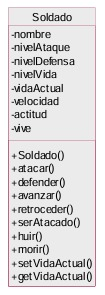
\includegraphics[height=10cm]{dia.jpeg}
        \subsubsection {Puede reutilizar todo el código del laboratorio 11, pero ahora el objetivo es gestionar los ejércitos autogenerados.}
        \subsubsection {Al ejecutar el videojuego, el programa deberá dar las opciones:}
        \paragraph {1. Juego rápido (tal cual como en el laboratorio 11) Al acabar el juego mostrar las opciones de volver a jugar y de volver al menú principal. También se deberá tener la posibilidad de cancelar el juego actual en cualquier momento, permitiendo escoger entre empezar un juego totalmente nuevo o salir al menú principal.}
        \paragraph {2. Juego personalizado: permite gestionar ejércitos. Primero se generan los 2 ejércitos con sus respectivos soldados y se muestran sus datos. Luego se tendrá que escoger cuál de los 2 ejércitos se va a gestionar, después se mostrarán las siguientes opciones:} 
            \subparagraph {2.1 Crear Soldado: permitirá crear un nuevo soldado personalizado y añadir al final del ejército (recordar que límite es de 10 soldados por ejército)}
        \subparagraph {2.2 Eliminar Soldado (no debe permitir un ejército vacío)} 
        \subparagraph {2.3 Clonar Soldado (crea una copia exacta del soldado) y se añade al final del ejército (recordar que límite es de 10 soldados por ejército)} 
        \subparagraph {2.4 Modificar Soldado (con submenú para cambiar alguno de los atributos nivelAtaque, nivelDefensa, vidaActual)} 
        \subparagraph {2.5 Comparar Soldados (verifica si atributos: nombre, nivelAtaque, nivelDefensa, vidaActual y vive son iguales)}
        \subparagraph {2.6 Intercambiar Soldados (intercambia 2 soldados en sus posiciones en la estructura de datos del ejército)} 
        \subparagraph {2.7 Ver soldado (Búsqueda por nombre)} 
        \subparagraph {2.8 Ver ejército} 
        \subparagraph {2.9 Sumar niveles (usando Method-Call Chaining), calcular las sumatorias de nivelVida, nivelAtaque, nivelDefensa, velocidad de todos los soldados de un ejército}
        \subparagraph {2.10 Jugar (se empezará el juego con los cambios realizados) y con las mismas opciones de la opción 1.}
        \subparagraph {2.11 Volver (muestra el menú principal) Después de escoger alguna de las opciones 1) a 9) se podrá volver a elegir uno de los ejércitos y se mostrarán las opciones 1) a 11)} 
        \paragraph 3. Salir
        \item la clase Main.java
        
        \begin{lstlisting}[language=java]
// RONI COMPANOCCA CHECCO
// CUI: 20210558
// LABORATORIO 12
import java.util.ArrayList;
import java.util.Collections;
import java.util.Comparator;

public class Main {

    public static void main(String[] args) {

		//DECLARACION DE VARIABLES Y ARREGLOS NECESARIOS
		ArrayList<Soldado> ejercito1 = new ArrayList();
		ArrayList<Soldado> ejercito2 = new ArrayList();
		ArrayList<ArrayList<Soldado>> tablero = new ArrayList();
		int batallon1, batallon2;
		int vidatotal1=0, vidatotal2=0;
		double promedioVida1=0, promedioVida2=0;

		// BUCLE PARA DESIGNAR LA CANTIDAD DE FILAS Y COLUMNAS DEL TABLERO
		for(int i=0; i<10; i++) {
			tablero.add(new ArrayList<Soldado>());
			for(int j=0; j<10; j++) {
				tablero.get(i).add(new Soldado());
			}
		}

		// CREACION DEL NUMERO DE POSICIONES DE CADA EJERCITO
		batallon1 = aleatorio(1,10);
		batallon2 = aleatorio(1,10);

		// INICIALIZAR ARREGLOS
		inicializarArreglo(ejercito1, batallon1);
		inicializarArreglo(ejercito2, batallon2);

		// GENERAR EJERCITOS VALIDOS
		generarEjercitos(ejercito1, ejercito2);

		// AÑADIR LOS EJERCITOS AL TABLERO
		añadirTablero(ejercito1, tablero);
		añadirTablero(ejercito2, tablero);

		//IMPRIMIR EL TABLERO
		imprimirTablero(tablero);

		//IMPRIMIR LOS SOLDADOS DE MAYOR VIDA DE CADA EJERCITO
		System.out.println("Soldado de mayor vida del ejercito 1");
		SoldadoConMayorVida(ejercito1);
		System.out.println("soldado de mayor vida del ejercito 2");
		SoldadoConMayorVida(ejercito2);

		//IMPRIMIR LA VIDA TOTAL Y EL PROMEDIO DEL EJERCITO 1
		System.out.println("\nEJERCITO 1: ");
		for (int i=0; i<ejercito1.size(); i++) {
			vidatotal1+=ejercito1.get(i).getPuntos();
			promedioVida1 = vidatotal1/(ejercito1.size()*1.0);
		}
		System.out.println("Vida total: "+vidatotal1);
		System.out.println("Promedio de vida: "+promedioVida1);
		
		//IMPRIMIR LA VIDA TOTAL Y EL PROMEDIO DEL EJERCITO 2
		System.out.println("\nEJERCITO 2: ");
		for (int i=0; i<ejercito2.size(); i++) {
			vidatotal2+=ejercito2.get(i).getPuntos();
			promedioVida2 = vidatotal2/(ejercito2.size()*1.0);
		}
		System.out.println("Vida total: "+vidatotal2);
		System.out.println("Promedio de vida: "+promedioVida2);

		//IMPRIMIR LOS SOLDADOS CREADOS EN EL ORDEN POR DEFECTO
		System.out.println("\nLista ejercito 1:");
		for(int i=0; i<ejercito1.size(); i++) {
			imprimir(ejercito1.get(i));
		}
		System.out.println("\nLista ejercito 2:");
		for(int i=0; i<ejercito2.size(); i++) {
			imprimir(ejercito2.get(i));
		}

		// IMPRIMIR LOS DATOS DE LOS SOLDADOS ORDENADOS DE MAYOR A MENOR DEPENDIENDO DE SU NIVEL DE VIDA USANDO DOS TIPOS DE ALGORITMO
		ordenarPorVidaMetodoA(ejercito1);
		ordenarPorVidaMetodoB(ejercito2);
		System.out.println("\nEjercito 1 Ordenados por nivel de vida");
		for(int i=0; i<ejercito1.size(); i++) {
			imprimir(ejercito1.get(i));
		}
		System.out.println("\nEjercito 2 Ordenados por nivel de vida");
		for(int i=0; i<ejercito2.size(); i++) {
			imprimir(ejercito2.get(i));
		}
		
		// MOSTRAR EJERCITO GANADOR LA METRICA USADA ARA DESIGNAR AL GANADOR ES POR EL NIVEL DEL PROMEDIO DE VIDA DE CADA EJERCITO
		if(promedioVida1>promedioVida2) {
			System.out.println("\nGANADOR ***EJERCITO 1***");
		}else if (promedioVida1<promedioVida2) {
			System.out.println("\nGANADOR ***EJERCITO 2***");
			}
		else {
			System.out.print("\n***ES UN EMPATE***");
		}
	}

    // METODO PARA CREAR NUMEROS ALEATORIOS EN UN RANGO
    public static int aleatorio(int min, int max) {
        return (int) (Math.random() * (max - min + 1) + min);
    }

    // METODO PARA INICIAR UN ARRAYLIST
    public static void inicializarArreglo(ArrayList<Soldado> soldadito, int num) {
        for (int i = 0; i < num; i++) {
            soldadito.add(new Soldado());
        }
    }

    // METODO PARA GENERAR DATOS DEL OBJETO SOLDADO
    public static Soldado generarDatos() {
        Soldado soldadito = new Soldado();
        soldadito.setNivelVida(aleatorio(1, 5));
        soldadito.setFila(aleatorio(1, 10));
        soldadito.setColumna(aleatorio(1, 10));
        return soldadito;
    }

    // METODOS PARA GENERAR LOS EJERCITOS DE MANERA ALEATORIA
    public static void generarEjercitos(ArrayList<Soldado> B1, ArrayList<Soldado> B2) {
        ArrayList<Soldado> Soldados = new ArrayList<>();
        Soldados.add(generarDatos());
        for (int i = 1; i < (B1.size() + B2.size()); i++) {
            Soldados.add(generarDatos());
            for (int j = 0; j < i; j++) {
                if (Soldados.get(i).getFila() == Soldados.get(j).getFila()) {
                    if (Soldados.get(i).getColumna() == Soldados.get(j).getColumna()) {
                        Soldados.remove(i);
                        i--;
                    }
                }
            }
        }
        for (int i = 0; i < B1.size(); i++) {
            B1.add(i, Soldados.get(i));
            B1.get(i).setNombre("Soldado" + i + "x1");
            B1.get(i).setActitud(B1.get(i).getNivelVida() + "[E1]");
            B1.remove(i + 1);
        }
        for (int i = 0; i < B2.size(); i++) {
            B2.add(i, Soldados.get(i + B1.size()));
            B2.get(i).setNombre("Soldado" + i + "x2");
            B2.remove(i + 1);
            B2.get(i).setActitud(B2.get(i).getNivelVida() + "[E2]");
        }
    }

    // METODO PARA AÑADIR LOS EJERCITOS AL TABLERO
    public static void añadirTablero(ArrayList<Soldado> soldadito, ArrayList<ArrayList<Soldado>> table) {
        for (int i = 0; i < soldadito.size(); i++) {
            table.get(soldadito.get(i).getColumna() - 1).add(soldadito.get(i).getFila() - 1, soldadito.get(i));
            table.get(soldadito.get(i).getColumna() - 1).remove(soldadito.get(i).getFila());
        }
    }

    // METODO PARA IMPRIMIR EL TABLERO EN LA CUAL SE DESARROLLA EL JUEGO
    public static void imprimirTablero(ArrayList<ArrayList<Soldado>> table) {
        System.out.println("\tA\tB\tC\tD\tF\tG\tH\tI\tJ");
        for (int i = 0; i < table.size(); i++) {
            System.out.print(i + 1);
            for (int j = 0; j < table.get(i).size(); j++) {
                System.out.print("\t" + table.get(i).get(j).getActitud());
            }
            System.out.println("\n");
        }
    }

    // METODO PARA IMPRIMIR LOS SOLDADOS DE MAYOR VIDA
    public static void SoldadoConMayorVida(ArrayList<Soldado> soldadito) {
        Soldado mayor = new Soldado();
        mayor.setNivelVida(0);
        for (int i = 0; i < soldadito.size(); i++) {
            if (mayor.getNivelVida() < soldadito.get(i).getNivelVida()) {
                mayor = soldadito.get(i);
            }
        }
        imprimir(mayor);
    }

    // METODO PARA IMPRIMIR EL NOMBRE, LA POSICION Y NIVEL DE VIDA DEL SOLDADO
    public static void imprimir(Soldado soldadito) {
        System.out.println("Nombre: " + soldadito.getNombre() + "\nPosicion: " + soldadito.getColumna() + "X" + soldadito.getFila() + "\tVida: " + soldadito.getNivelVida());
    }

    // METODO QUE NOS AYUDA A ORDENAR LOS SOLDADOS DE ACUERDO A SU NIVEL DE VIDA, USUANDO UN ALGORITMO DE ORDENAMIENTO DE BURBUJA
    public static void ordenarPorVidaMetodoA(ArrayList<Soldado> soldadito) {
        Soldado aux = new Soldado();
        for (int i = 0; i < soldadito.size() - 1; i++) {
            for (int j = 0; j < soldadito.size() - i - 1; j++) {
                if (soldadito.get(j).getNivelVida() < soldadito.get(j + 1).getNivelVida()) {
                    aux = soldadito.get(j);
                    soldadito.set(j, soldadito.get(j + 1));
                    soldadito.set(j + 1, aux);
                }
            }
        }
    }

    // METODO QUE NOS AYUDA A ORDENAR LOS SOLDADOS DE ACUERDO A SU NIVEL DE VIDA, EN ESTA OCACION DIFERENTE A LA ANTERIOR QUE ERA ALGORITMO DE BURBUJA
    public static void ordenarPorVidaMetodoB(ArrayList<Soldado> soldadito) {
        Collections.sort(soldadito, new Comparator<Soldado>() {
            public int compare(Soldado s1, Soldado s2) {
                // Orden descendente por nivel de vida
                return Integer.compare(s2.getNivelVida(), s1.getNivelVida());
            }
        });
    }
}
    // METODO PARA IMPRIMIR EL TABLERO EN LA CUAL SE DESARROLLA EL JUEGO
    public static void imprimirTablero(ArrayList<ArrayList<Soldado>> table) {
        System.out.println("\tA\tB\tC\tD\tF\tG\tH\tI\tJ");
        for (int i = 0; i < table.size(); i++) {
            System.out.print(i + 1);
            for (int j = 0; j < table.get(i).size(); j++) {
                System.out.print("\t" + table.get(i).get(j).getActitud());
            }
            System.out.println("\n");
        }
    }

    // METODO PARA IMPRIMIR LOS SOLDADOS DE MAYOR VIDA
    public static void SoldadoConMayorVida(ArrayList<Soldado> soldadito) {
        Soldado mayor = new Soldado();
        mayor.setNivelVida(0);
        for (int i = 0; i < soldadito.size(); i++) {
            if (mayor.getNivelVida() < soldadito.get(i).getNivelVida()) {
                mayor = soldadito.get(i);
            }
        }
        imprimir(mayor);
    }

    // METODO PARA IMPRIMIR EL NOMBRE, LA POSICION Y NIVEL DE VIDA DEL SOLDADO
    public static void imprimir(Soldado soldadito) {
        System.out.println("Nombre: " + soldadito.getNombre() + "\nPosicion: " + soldadito.getColumna() + "X" + soldadito.getFila() + "\tVida: " + soldadito.getNivelVida());
    }

    // METODO QUE NOS AYUDA A ORDENAR LOS SOLDADOS DE ACUERDO A SU NIVEL DE VIDA, USUANDO UN ALGORITMO DE ORDENAMIENTO DE BURBUJA
    public static void ordenarPorVidaMetodoA(ArrayList<Soldado> soldadito) {
        Soldado aux = new Soldado();
        for (int i = 0; i < soldadito.size() - 1; i++) {
            for (int j = 0; j < soldadito.size() - i - 1; j++) {
                if (soldadito.get(j).getNivelVida() < soldadito.get(j + 1).getNivelVida()) {
                    aux = soldadito.get(j);
                    soldadito.set(j, soldadito.get(j + 1));
                    soldadito.set(j + 1, aux);
                }
            }
        }
    }

    // METODO QUE NOS AYUDA A ORDENAR LOS SOLDADOS DE ACUERDO A SU NIVEL DE VIDA, EN ESTA OCACION DIFERENTE A LA ANTERIOR QUE ERA ALGORITMO DE BURBUJA
    public static void ordenarPorVidaMetodoB(ArrayList<Soldado> soldadito) {
        Collections.sort(soldadito, new Comparator<Soldado>() {
            public int compare(Soldado s1, Soldado s2) {
                // Orden descendente por nivel de vida
                return Integer.compare(s2.getNivelVida(), s1.getNivelVida());
            }
        });
    }
}
        \end{lstlisting}

        \item la clase Soldado.java
        \begin{lstlisting}[language=java]
// RONI COMPANOCCA CHECCO
// CUI: 20210558
// LABORATORIO 12
// FUNDAMENTOS DE PROGRAMACION 
// CLASE SOLDADO PARA LOS METODOS SETTER Y GETTER
public class Soldado {
    private String nombre;
    private int nivelAtaque;
    private int nivelDefensa;
    private int nivelVida;
    private int vidaActual;
    private int velocidad;
    private String actitud;
    private boolean vive;

    public Soldado() {
        nombre = "";
        nivelAtaque = 0;
        nivelDefensa = 0;
        nivelVida = 0;
        vidaActual = nivelVida;
        velocidad = 0;
        actitud = "";
        vive = true;
    }

    public void atacar(Soldado enemigo) {
        int danio = this.nivelAtaque - enemigo.nivelDefensa;
        if (danio > 0) {
            enemigo.serAtacado(danio);
            System.out.println(this.nombre + " atacó a " + enemigo.nombre + " y le causó " + danio + " de daño.");
        } else {
            System.out.println(this.nombre + " atacó a " + enemigo.nombre + " pero no le causó daño.");
        }
    }

    public void defender() {
        // Lógica para la defensa
        // Puede disminuir el daño recibido en un futuro ataque, por ejemplo
        this.nivelDefensa += 10; // Aumentar la defensa por ejemplo
        System.out.println(this.nombre + " se está defendiendo.");
    }

    public void avanzar() {
        // Lógica para avanzar en el juego
        // Podría mover al soldado a una nueva posición en el tablero, por ejemplo
        if (this.velocidad > 0) {
            // Mover al soldado en la dirección correspondiente
            System.out.println(this.nombre + " está avanzando.");
        } else {
            System.out.println(this.nombre + " no puede avanzar, la velocidad es 0.");
        }
    }

    public void retroceder() {
        // Lógica para retroceder en el juego
        // Podría mover al soldado hacia atrás en el tablero, por ejemplo
        System.out.println(this.nombre + " está retrocediendo.");
    }

    public void serAtacado(int danioRecibido) {
        this.vidaActual -= danioRecibido;
        if (this.vidaActual <= 0) {
            this.morir();
        }
    }

    public void huir() {
        // Lógica para huir del combate
        // Podría cambiar la posición del soldado a una zona segura, por ejemplo
        if (this.nivelVida < 10) {
            // Huir solo si la vida es baja
            System.out.println(this.nombre + " está huyendo del combate.");
        } else {
            System.out.println(this.nombre + " no puede huir, su vida está alta.");
        }
    }

    public void morir() {
        this.vidaActual = 0;
        this.vive = false;
    }

    public void setVidaActual(int vidaActual) {
        this.vidaActual = vidaActual;
    }

    public int getVidaActual() {
        return vidaActual;
    }

    // Getters y Setters

    public String getNombre() {
        return nombre;
    }

    public String getNivelVida() {
        return nivelVida;
    }

    public void setNombre(String nombre) {
        this.nombre = nombre;
    }

    public int getNivelAtaque() {
        return nivelAtaque;
    }

    public int setNivelVida() {
        this.nivelVida = nivelVida;
    }

    public void setNivelAtaque(int nivelAtaque) {
        this.nivelAtaque = nivelAtaque;
    }

    public int getNivelDefensa() {
        return nivelDefensa;
    }

    public void setNivelDefensa(int nivelDefensa) {
        this.nivelDefensa = nivelDefensa;
    }

    public boolean isVive() {
        return vive;
    }

    public void setVive(boolean vive) {
        this.vive = vive;
    }
}
        \end{lstlisting}

        
        \item Ejecucion
        \begin{lstlisting}[language=java]
            A       B       C       D       F       G       H       I       J
1                                               2[E1]

2                                                               5[E1]

3

4

5

6                                                                       2[E2]

7

8                               2[E1]   3[E2]

9       3[E2]                                                           2[E1]

10                                              2[E1]           3[E2]

Soldado de mayor vida del ejercito 1
Nombre: Soldado4x1
Posicion: 2X8   Vida: 5
soldado de mayor vida del ejercito 2
Nombre: Soldado0x2
Posicion: 10X8  Vida: 3

EJERCITO 1:
Vida total: 13
Promedio de vida: 2.6

EJERCITO 2:
Vida total: 11
Promedio de vida: 2.75

Lista ejercito 1:
Nombre: Soldado0x1
Posicion: 1X6   Vida: 2
Nombre: Soldado1x1
Posicion: 9X9   Vida: 2
Nombre: Soldado2x1
Posicion: 8X4   Vida: 2
Nombre: Soldado3x1
Posicion: 10X6  Vida: 2
Nombre: Soldado4x1
Posicion: 2X8   Vida: 5

Lista ejercito 2:
Nombre: Soldado0x2
Posicion: 10X8  Vida: 3
Nombre: Soldado1x2
Posicion: 8X5   Vida: 3
Nombre: Soldado2x2
Posicion: 6X9   Vida: 2
Nombre: Soldado3x2
Posicion: 9X1   Vida: 3

Ejercito 1 Ordenados por nivel de vida
Nombre: Soldado4x1
Posicion: 2X8   Vida: 5
Nombre: Soldado0x1
Posicion: 1X6   Vida: 2
Nombre: Soldado1x1
Posicion: 9X9   Vida: 2
Nombre: Soldado2x1
Posicion: 8X4   Vida: 2
Nombre: Soldado3x1
Posicion: 10X6  Vida: 2

Ejercito 2 Ordenados por nivel de vida
Nombre: Soldado0x2
Posicion: 10X8  Vida: 3
Nombre: Soldado1x2
Posicion: 8X5   Vida: 3
Nombre: Soldado3x2
Posicion: 9X1   Vida: 3
Nombre: Soldado2x2
Posicion: 6X9   Vida: 2

GANADOR ***EJERCITO 2***
        \end{lstlisting}

    
	\end{itemize}
	
	\section{REFERENCIAS}
	\begin{itemize}
		\item M. Aedo, “Fundamentos de Programación 2 - Tópicos de Programación Orientada a Objetos”, Primera Edición, 2021, Editorial UNSA.
		\item \url{https://github.com/rescobedoq/programacion.git}
		\item J. Dean, "Introduction to programming with Java: A Problem Solving Approach”, Third Edition, 2021, McGraw-Hill.
        \item C. T. Wu, "An Introduction to Object-Oriented Programming with Java", Fifth Edition, 2010, McGraw-Hill.
        \item P. Deitel, "Java How to Program", Eleventh Edition, 2017, Prentice Hall.
	\end{itemize}
	
%\clearpage
%\bibliographystyle{apalike}
%\bibliographystyle{IEEEtranN}
%\bibliography{bibliography}
			
\end{document}